%====================================================================
% EC8203 Applied Big Data Engineering -- Mini-Project Report
% Fleet Operations: A Lambda-Architecture Data Pipeline
% Department of Electrical and Information Engineering,
% Faculty of Engineering, University of Ruhuna
%
% Build:  make report
%    or:  pdflatex report && bibtex report && pdflatex report && pdflatex report
%
% Page geometry, header/footer and front-matter order follow the DEIE
% report template (pagesetup.cfg). Do not change them to fit content --
% shorten the content instead.
%====================================================================
\documentclass[a4paper,12pt]{report}

\usepackage[T1]{fontenc}
\usepackage[utf8]{inputenc}
\usepackage{graphicx}
\usepackage{amsmath}
\usepackage{amssymb}
\usepackage{listings}
\usepackage{multicol}
\usepackage{fancyhdr}
\usepackage{lastpage}
\usepackage{longtable}
\usepackage{booktabs}
\usepackage{tabularx}
\usepackage{xcolor}

% A stretchy right-aligned column. tabularx needs at least one X column to
% have something to stretch; an all-fixed table silently overruns the margin
% instead of wrapping, which is how the four-day results table ended up two
% inches wide of the text block.
\newcolumntype{R}{>{\raggedleft\arraybackslash}X}

%--------------------------------------------------------------------
% Density. This report is a mini-project bound by a 10-13 page target
% overall. These values
% tighten the gaps around lists, tables and floats without touching
% line spacing, font size or margins, all of which the DEIE template
% fixes and none of which may be altered.
%--------------------------------------------------------------------
\usepackage{enumitem}
\setlist{topsep=2pt, itemsep=1pt, parsep=0pt, partopsep=0pt}
\setlist[description]{topsep=3pt, itemsep=2pt}

\renewcommand{\arraystretch}{0.95}
\setlength{\tabcolsep}{4pt}

% Tables already set \small in their own source; this takes them one
% size further without editing each environment, and re-points \small
% inside a table so those local declarations do not undo it.
\usepackage{etoolbox}
\AtBeginEnvironment{table}{\footnotesize\let\small\footnotesize}
\AtBeginEnvironment{longtable}{\footnotesize\let\small\footnotesize}

% tocloft is loaded before hyperref, which is the order those two require.
\usepackage{tocloft}
\setlength{\cftbeforechapskip}{2pt}
\setlength{\cftbeforesecskip}{0pt}
\setlength{\cftbeforesubsecskip}{0pt}
\setlength{\cftbeforefigskip}{0pt}
\setlength{\cftbeforetabskip}{0pt}
\renewcommand{\cftchapfont}{\bfseries}
% Contents, figures and tables share one page, so their titles are smaller
% and closer together than tocloft's chapter-sized defaults.
\renewcommand{\cfttoctitlefont}{\LARGE\bfseries}
\renewcommand{\cftloftitlefont}{\LARGE\bfseries}
\renewcommand{\cftlottitlefont}{\LARGE\bfseries}
\setlength{\cftbeforetoctitleskip}{0pt}
\setlength{\cftbeforeloftitleskip}{12pt}
\setlength{\cftbeforelottitleskip}{12pt}
\setlength{\cftaftertoctitleskip}{8pt}
\setlength{\cftafterloftitleskip}{8pt}
\setlength{\cftafterlottitleskip}{8pt}
\renewcommand{\cftchappagefont}{\bfseries}

\setlength{\textfloatsep}{10pt plus 2pt minus 2pt}
\setlength{\floatsep}{8pt plus 2pt minus 2pt}
\setlength{\intextsep}{8pt plus 2pt minus 2pt}
\setlength{\abovecaptionskip}{4pt}
\setlength{\belowcaptionskip}{0pt}

% Let a float share a page with less text around it, rather than being
% deferred and leaving part-empty pages behind it.
\renewcommand{\topfraction}{0.9}
\renewcommand{\bottomfraction}{0.8}
\renewcommand{\textfraction}{0.07}
\renewcommand{\floatpagefraction}{0.8}

% A chapter opening drops ~2 in of white space in report.cls.
\usepackage{titlesec}
\titlespacing*{\chapter}{0pt}{-20pt}{18pt}

% report.cls forces every \chapter onto a fresh page. That is right for a
% 100-page thesis and wrong for a mini-project the brief caps at 8-15 pages:
% five forced breaks plus five part-empty closing pages cost about three
% pages of white paper, which would otherwise have to come out of the
% argument. Chapters now flow on the page and keep their "Chapter N" heading
% style. \needspace stops a heading being orphaned at the foot of a page.
\usepackage{needspace}
\makeatletter
\renewcommand\chapter{%
  \par\addvspace{2.5\baselineskip}%
  \needspace{6\baselineskip}%
  \global\@topnum\z@
  \@afterindentfalse
  \secdef\@chapter\@schapter}
\makeatother
\titlespacing*{\section}{0pt}{2.2ex plus 0.6ex minus 0.2ex}{1.2ex plus 0.2ex}
\titlespacing*{\subsection}{0pt}{1.8ex plus 0.5ex minus 0.2ex}{0.8ex plus 0.2ex}

%--------------------------------------------------------------------
% Page set-up (values from the DEIE report template, pagesetup.cfg)
%--------------------------------------------------------------------
\setlength{\oddsidemargin}{0.25in}
\setlength{\evensidemargin}{0.25in}
\setlength{\topmargin}{-0.5in}
\setlength{\headheight}{22.5pt}
\setlength{\headsep}{0.25in}
\setlength{\topskip}{0cm}
\setlength{\textwidth}{6in}
\setlength{\textheight}{9.7in}
\setlength{\footskip}{0.75in}

% Extra inter-word stretch, so the many unbreakable \texttt identifiers
% (metric names, table names) do not overflow the margin.
\setlength{\emergencystretch}{3em}
\raggedbottom

\pagestyle{fancy}
\fancyhf{}
\lhead{\footnotesize\leftmark}
\cfoot{Page \thepage\ of \pageref{LastPage}}
\renewcommand{\headrulewidth}{0.4pt}
\renewcommand{\footrulewidth}{0pt}

%--------------------------------------------------------------------
% Links
%--------------------------------------------------------------------
\usepackage[breaklinks]{hyperref}
\hypersetup{colorlinks=true,citecolor=blue,linkcolor=blue,urlcolor=blue}
\usepackage{url}
\def\UrlBreaks{\do\/\do\-\do\_}

%--------------------------------------------------------------------
% Code listing style
%--------------------------------------------------------------------
\definecolor{codegray}{gray}{0.95}
\definecolor{codekw}{rgb}{0.0,0.2,0.6}
\definecolor{codestr}{rgb}{0.55,0.10,0.10}
\definecolor{codecom}{rgb}{0.25,0.50,0.25}
\lstset{
  backgroundcolor=\color{codegray},
  basicstyle=\ttfamily\scriptsize,
  keywordstyle=\color{codekw}\bfseries,
  stringstyle=\color{codestr},
  commentstyle=\color{codecom}\itshape,
  showstringspaces=false,
  breaklines=true,
  frame=single,
  framerule=0.3pt,
  aboveskip=6pt,
  belowskip=6pt,
  xleftmargin=10pt,
  language=Python
}

%--------------------------------------------------------------------
% Shorthands. \code is used for every identifier, table, metric and
% file path in the report; it takes a verbatim-ish argument so the
% underscores in metric names do not need escaping at each use.
%--------------------------------------------------------------------
% Identifiers such as test_spark_validation_matches_the_python_rules are a
% single unbreakable word to TeX, and in a narrow tabularx column they run
% two inches past the margin. Redefining \_ inside \code to carry an
% \allowbreak gives TeX a legal break after every underscore. No hyphen is
% inserted, which matters: a hyphen would read as part of the identifier.
\newcommand{\code}[1]{{\def\_{\textunderscore\allowbreak}\texttt{\small #1}}}

\begin{document}

%====================================================================
% COVER PAGE
%====================================================================
\thispagestyle{empty}
\begin{center}


\includegraphics[width=2cm,keepaspectratio=true]{uor_logo.jpg}

\vspace{0.8cm}
\begin{huge}
\textbf{Fleet Operations:}\\[0.3cm]
\textbf{A Lambda-Architecture Data}\\
\textbf{Pipeline for Ride-Hailing}\\
\textbf{Utilisation and Profitability}
\end{huge}\\[0.5cm]

\begin{large}
\emph{answering a live question and a financial question
from one immutable master dataset}
\end{large}\\[0.9cm]

\begin{normalsize}
A mini-project report submitted to the
\end{normalsize}\\[0.5cm]

\begin{large}
Department of Electrical and Information Engineering\\
Faculty of Engineering\\
University of Ruhuna\\
Sri Lanka
\end{large}\\[0.7cm]

\begin{normalsize}in partial fulfilment of the requirements of\end{normalsize}\\[0.5cm]

\begin{large}\textbf{EC8203 --- Applied Big Data Engineering}\end{large}\\[0.7cm]

\begin{normalsize}by\end{normalsize}\\[0.4cm]

\begin{tabular}[h]{lll}
Ahamed N.F.F. & - & EG/2021/4390\\
Safeer S.M.   & - & EG/2021/4771\\
Nafla M.N.P.  & - & EG/2021/4687\\
\end{tabular}\\[1.2cm]

\begin{normalsize}
Use Case 1: Ride-Hailing Fleet Operations\\
Academic Year 2026 \quad\textbar\quad Mini-Project Report
\end{normalsize}

\end{center}

\clearpage

\renewcommand{\thepage}{\roman{page}}
\setcounter{page}{1}

%====================================================================
% CONTENTS, FIGURES, TABLES
%====================================================================
\setcounter{tocdepth}{1}
\setcounter{secnumdepth}{2}
{\small
\tableofcontents
\listoffigures
\listoftables
}
\clearpage

%====================================================================
%                       MAIN MATTER
%====================================================================
\renewcommand{\thepage}{\arabic{page}}
\setcounter{page}{1}

\chapter{Introduction}
\label{ch:introduction}

A ride-hailing operator runs two businesses at once: an operations
business conducted minute by minute (where are the cars, which are
earning, which have been idle for an hour) and a financial business
conducted a day at a time (what did each vehicle earn and cost, and is
it still worth running). This project builds one platform that answers
both without letting the fast answer contaminate the exact one.

\section{Problem Statement}
\label{sec:problem}

The brief specifies two ingestion paths. A \textbf{streaming source}
emits GPS and telemetry per vehicle every few seconds (\code{trip\_id},
\code{driver\_id}, \code{vehicle\_id}, position, speed, status, fare,
timestamp). A \textbf{daily batch source} drops one file per simulated
day of expense records from garages and fuel partners
(\code{vehicle\_id}, \code{fuel\_cost}, \code{maintenance\_cost},
\code{distance\_covered}, \code{service\_flag}). The telemetry is
high-volume and tolerant of small losses; the expense file is owned by a
third party, \emph{authoritative about money}, and can be corrected and
resubmitted days later, forcing published figures to be restated.

The business question --- \emph{what is utilisation and earnings by area
right now, and which vehicles are becoming unprofitable once yesterday's
costs are applied?} --- is really two questions with conflicting
requirements (Table~\ref{tab:two-questions}).

\begin{table}[htbp]
\centering
\caption{The two sub-questions and their incompatible requirements.}
\label{tab:two-questions}
\begin{tabularx}{\textwidth}{@{}lXX@{}}
\toprule
& \textbf{Live utilisation} & \textbf{Daily profitability}\\
\midrule
Latency       & seconds & next morning is acceptable\\
Accuracy      & approximate is fine & exact; it is money\\
Recomputable? & no need & \textbf{yes}; partners resubmit files\\
Consumer      & dispatcher watching a map & finance, making
                retire/keep decisions\\
\bottomrule
\end{tabularx}
\end{table}

\section{Objectives and Scope}
\label{sec:objectives}

The objectives were to choose between Lambda and Kappa on the evidence of
this use case; to simulate both sources with injected faults so error
handling is demonstrated rather than claimed; to perform real processing
(cleaning, zone enrichment, windowed aggregation, stateful alerting and a
cross-source join); to serve results through a store, API, dashboards and
a daily report; and to instrument every stage, including the pipeline's
\emph{known imprecision}.

The whole system runs on one 16\,GB laptop from one command, which forces
three simplifications: simulated time is compressed 60-fold
(Section~\ref{sec:simclock}), Kafka is a single broker at replication
factor~1, and batch Spark runs in local mode. Authentication is out of
scope.

\chapter{Architecture and Technology Stack}
\label{ch:architecture}

\section{Background: Lambda and Kappa}
\label{sec:lit-lambda}

Lambda (Marz and Warren) combines an \emph{immutable master dataset}, a
\emph{batch layer} that recomputes exact views from it, and a \emph{speed
layer} that computes approximate views over recent data. Because batch
views are a pure function of immutable input, errors are repaired by
recomputing, and the speed layer's error is temporary by construction.
Kreps's critique is that Lambda needs two implementations of every
business rule, which can drift apart; his alternative, Kappa, keeps one
stream processor and recomputes by \emph{replaying the log}. That works
only if everything needed to recompute a result is \emph{in the log} ---
the assumption this use case breaks.

Three stream-processing results underpin the correctness argument:
event time (when something happened) must be separated from processing
time; a \textbf{watermark is a bet}, and events later than it are
dropped, not deferred; and Spark's exactly-once guarantee stops at the
sink, so external writes from \code{foreachBatch} are at-least-once
unless the sink is idempotent.

\section{The Decision: Lambda}
\label{sec:decision}

We implement Lambda: an archiver writes the immutable master dataset, a
speed layer computes live views, and a batch layer recomputes exact
views from the archive (Figure~\ref{fig:architecture}).

\begin{figure}[htbp]
\centering
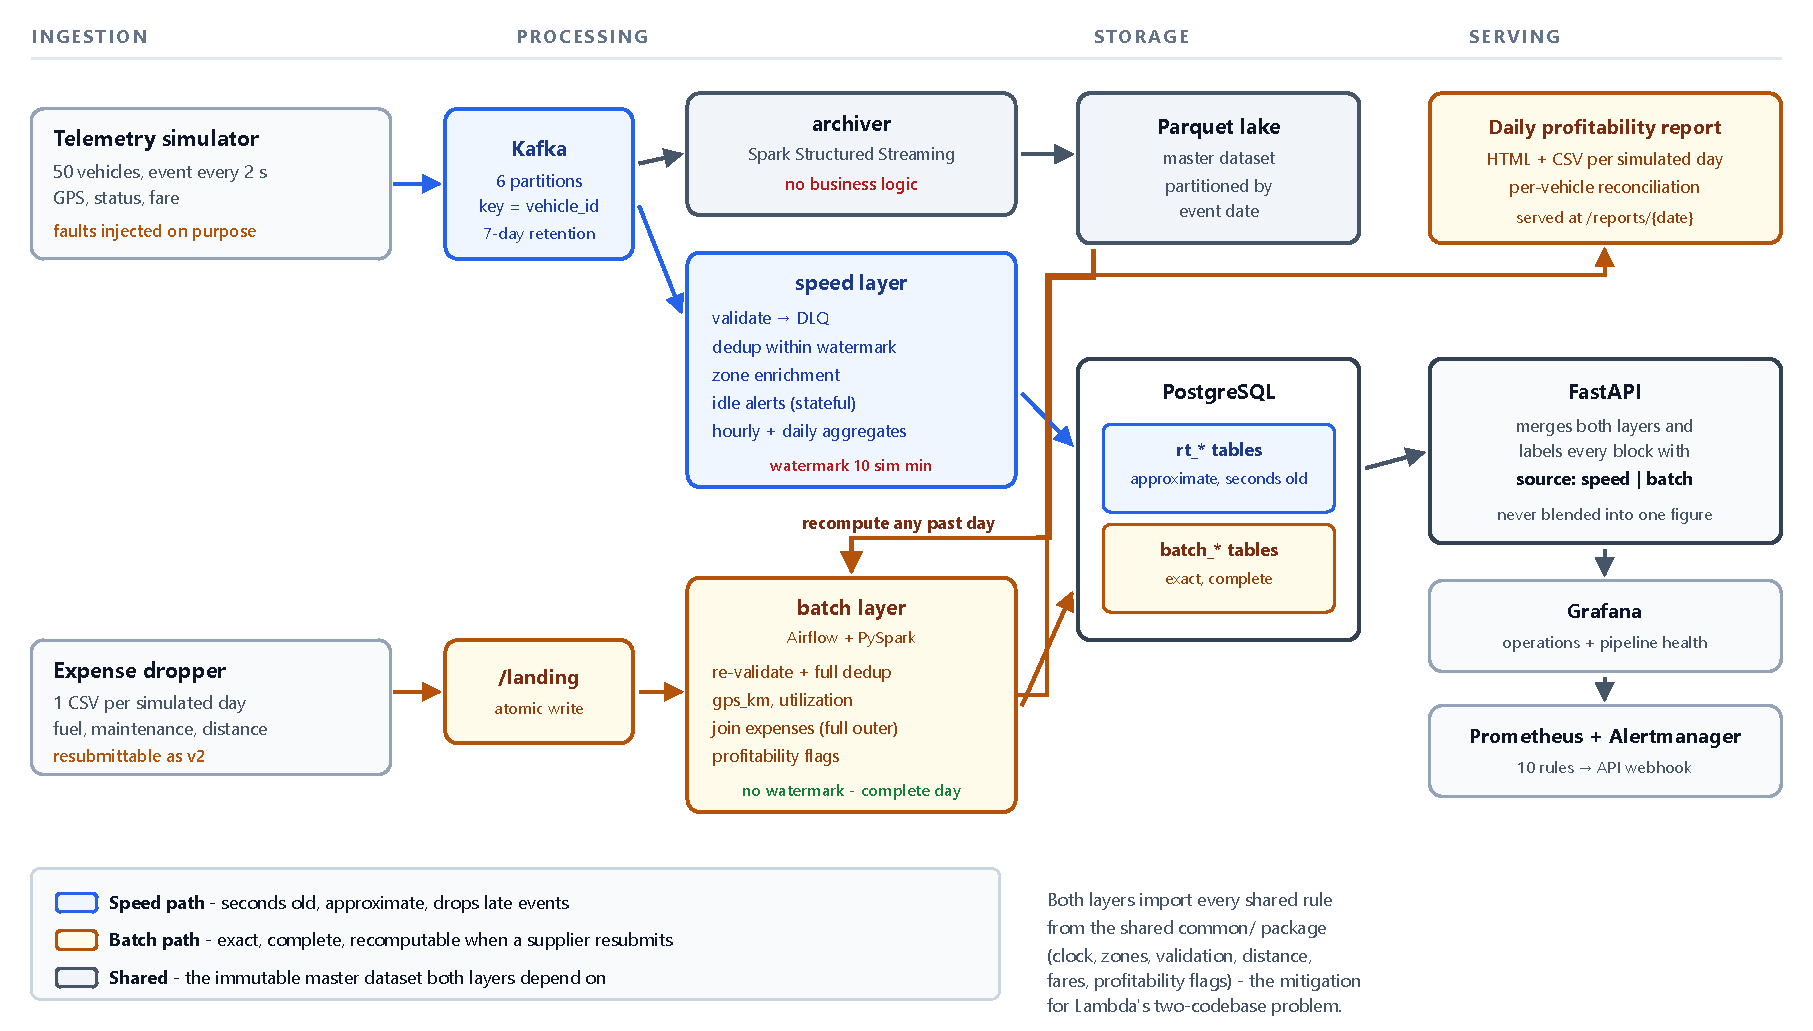
\includegraphics[width=0.95\textwidth]{figures/fig1-architecture.pdf}
\caption[System architecture]{System architecture. Blue: speed layer
(seconds old, approximate). Amber: batch layer (exact, recomputable).
Both read the same master dataset and import shared rules from
\code{common/}.}
\label{fig:architecture}
\end{figure}

\section{Why Kappa Was Rejected}
\label{sec:kappa-rejected}

The requirement is to \emph{restate a past day's financial figures} when
a partner sends corrected costs. Under Kappa:

\begin{enumerate}
  \item \textbf{Retention must cover any day we might restate} ---
        months of Kafka retention. Ours is \textbf{7 days}, enough for
        speed-layer recovery only.
  \item \textbf{Replay is not selective.} A Parquet lake partitioned by
        \code{sim\_date} lets the batch job read one partition; a full
        simulated day is computed in \textbf{9.4 seconds}.
  \item \textbf{The correction is not in the stream at all.} It arrives
        as a CSV file on a separate channel, so replaying the log does
        not touch what actually forces a restatement. Publishing the
        file to a topic only moves the problem back to point~1.
\end{enumerate}

A batch-only design was rejected because it cannot say which vehicles
are idle \emph{now}.

\section{What Lambda Costs, and Our Mitigation}
\label{sec:lambda-cost}

We accept Kreps's criticism and answer it structurally. A shared
\code{common/} package holds every rule both layers need --- simulated
clock, zone mapping, validation, haversine distance, fare maths and the
seven profitability flags --- and is imported by the simulators, both
processing layers and the API. Only two rules are duplicated, to avoid a
per-row Python UDF: validation (\code{validate\_event()} vs.\
\code{spark\_validation\_expr()}) and haversine distance. Each pair is
held in step by a test that feeds identical inputs to both.

\section{Technology Stack}
\label{sec:tech-stack}

Every image and package version is pinned (Table~\ref{tab:stack}).

\begin{table}[htbp]
\centering
\caption{Technology selection and the reason for each choice.}
\label{tab:stack}
\begin{tabularx}{\textwidth}{@{}llX@{}}
\toprule
\textbf{Layer} & \textbf{Choice} & \textbf{Why}\\
\midrule
Ingestion & Kafka 3.8 (KRaft) &
  Per-partition ordering is a correctness requirement; KRaft drops
  ZooKeeper.\\
Speed layer & Spark Structured Streaming 3.5.3 &
  Watermarks, windows and \code{applyInPandasWithState}; one engine for
  both layers makes \code{common/} shareable (preferred over Flink for
  that reason).\\
Master dataset & Parquet on a volume &
  Columnar, date-partitioned; paths built from \code{LAKE\_ROOT}, so
  moving to S3 is one variable.\\
Batch & Airflow 2.10 + PySpark &
  Retries, dependency ordering, per-task visibility; local mode suits
  $\sim$12k events/day.\\
Serving & PostgreSQL 16, FastAPI &
  Upserts on natural keys give idempotent sinks; Pydantic models make the
  \code{source} label part of the schema.\\
Observability & Prometheus, Alertmanager, Grafana &
  Pull-based metrics, routed alerts, dashboards.\\
\bottomrule
\end{tabularx}
\end{table}

\section{The Simulated Clock and Data Contract}
\label{sec:simclock}

\textbf{One real second is one simulated minute} (\code{COMPRESSION=60}),
so a simulated day takes 24 real minutes and a daily reconciliation can
be shown in a lab session. The clock is derived from a persisted start
instant, so every service agrees on \code{sim\_time} and restarts do not
rewind it.

We added three telemetry fields: \code{event\_id} (UUID, for
deduplication), \code{schema\_version}, and \code{event\_type}
(\code{ping}/\code{trip\_start}/\code{trip\_end}), which makes ``trips
completed'' a simple count instead of a chained stateful operator.
\textbf{\code{fare} is cumulative and final only on \code{trip\_end}}, so
revenue is \code{SUM(fare) WHERE event\_type='trip\_end'} in both layers.

\chapter{Implementation}
\label{ch:implementation}

\section{Ingestion}
\label{sec:impl-ingestion}

\subsection{Partitioning Is a Correctness Decision}
\label{sec:impl-partitioning}

The topic \code{fleet.telemetry} has 6 partitions, \textbf{keyed by
\code{vehicle\_id}}. Throughput has nothing to do with it. Kafka
guarantees ordering only \emph{within} a
partition~\cite{kreps2011kafka}, and the speed layer's per-vehicle state
machine, which tracks when each vehicle last went idle, assumes it sees
one vehicle's events in the order they happened. Keying by
\code{vehicle\_id} is what gives it that. Key round-robin instead and
every idle measurement quietly goes wrong, without anything anywhere
raising an error. The dead-letter topic \code{fleet.telemetry.dlq} has one
partition, since it needs no ordering and one partition keeps every
rejected event in a single readable stream.

\subsection{Fault Injection}
\label{sec:impl-faults}

The simulator corrupts its own output, so we can show the error handling
working rather than claim it does. Table~\ref{tab:faults} gives
configured against measured rates over roughly 2,700 events. Validation
rejects rather than repairs: coerce a malformed field and you
get a confidently wrong money figure downstream, which is worse than a
rejection somebody can see. The DLQ carries the reason code \emph{and the
original payload}, so once a producer is fixed its rejected events can be
replayed. The observed distribution was \code{unparseable\_json}~58,
\code{coords\_out\_of\_bounds}~23, \code{bad\_status}~17,
\code{negative\_fare}~12 and \code{negative\_speed}~10.

\begin{table}[htbp]
\centering
\caption{Injected fault rates, configured against measured, and what each
fault demonstrates.}
\label{tab:faults}
\begin{tabularx}{\textwidth}{@{}llrX@{}}
\toprule
\textbf{Fault} & \textbf{Config.} & \textbf{Measured} &
\textbf{What it proves}\\
\midrule
Malformed JSON & 0.5\% & 0.40\% &
  The archiver preserves unparseable bytes; the speed layer
  dead-letters rather than crashing\\
Schema-invalid & 0.5\% & 0.77\% &
  \code{common/validation.py} rejects identically in both layers\\
Duplicate \code{event\_id} & 1.0\% & 1.03\% &
  Deduplication works; both copies are \emph{valid}, so nothing else
  can stop them\\
Late by 1--20 sim min & 2.0\% & 2.09\% &
  The consistency argument; see Section~\ref{sec:consistency}\\
\bottomrule
\end{tabularx}
\end{table}

A second simulator drops one expense CSV per simulated day. Files are
versioned, so a partner correcting an earlier submission drops a
\code{v2} file for a date already reconciled. That is the event the whole
architecture exists to absorb (Section~\ref{sec:recompute}). The delivery
SLA governs first delivery only. An early version checked it
against every version, which meant a corrected \code{v2} marked every
resubmission late.

\section{The Speed Layer}
\label{sec:impl-speed}

\subsection{The Archiver Does as Little as Possible}
\label{sec:impl-archiver}

The archiver is a \emph{separate Spark application} with its own
checkpoint and \textbf{no business logic at all}. Every past day is
recomputed from the master dataset, so if the master dataset is corrupt
then all history is wrong and nothing can recover it. Keeping the
archiver separate means a bug in the speed layer's validation, windowing
or state handling \emph{cannot reach it}. The worst such a bug can do is
produce wrong dashboards, and the next batch run overwrites those.
Unparseable records are archived under \code{sim\_date=unknown} with
their raw bytes intact. An archive that quietly dropped them would make
``how much bad data did we receive?'' unanswerable forever.

\subsection{Stateful Idle Alerts}
\label{sec:impl-idle}

No window or aggregation can answer ``has this vehicle been idle for 45
simulated minutes?''. Answering it needs memory of \emph{when} the
vehicle last stopped being idle, carried across micro-batches, plus the
ability to fire when no new event arrives at all, since a silent
vehicle is exactly the case we care about.
\code{applyInPandasWithState} is the only Structured Streaming construct
that offers both~\cite{spark_ss_guide}. Four details decide whether it
works, and each is a defect if you get it wrong:

\begin{enumerate}
  \item \textbf{The stopwatch starts on the \emph{transition} into
        idle}, not on every idle ping. Resetting per ping means the timer
        never advances and no alert can fire.
  \item \textbf{Events are sorted by event time before folding}, because
        a micro-batch may interleave partitions.
  \item \textbf{A stale out-of-order event does not rewind the state.}
        The event is not lost, since the archive holds it and the batch
        layer counts it, but rewinding would corrupt the idle
        measurement.
  \item \textbf{\code{EventTimeTimeout}, not
        \code{ProcessingTimeTimeout}.} A processing-time timeout fires
        after $N$ \emph{real} seconds, so changing the clock compression
        would silently change the business rule.
\end{enumerate}

This design has a consequence we would rather state than hide. An
event-time timeout fires only when the watermark advances, and the
watermark advances only when other events
arrive~\cite{akidau2015dataflow}. If the whole fleet went silent at once,
no timeout would fire at all. A different control covers that case: the
\code{TelemetryNotProduced} alert, which watches the producer directly.

\subsection{Idempotent Sinks}
\label{sec:impl-sinks}

\code{foreachBatch} gives \textbf{at-least-once} delivery. If the driver
dies after writing a micro-batch but before committing offsets, Spark
re-runs the batch and the sink sees the same rows
twice~\cite{armbrust2018structured}. With plain inserts, every dashboard
figure would ratchet upward on each restart and never come back down.
Every sink therefore upserts on a natural key:
\code{rt\_vehicle\_state} on \code{(vehicle\_id)},
\code{rt\_zone\_hourly} on \code{(zone\_id, window\_start)},
\code{rt\_vehicle\_daily} on \code{(vehicle\_id, sim\_date)}, and
\code{idle\_alerts} on \code{(vehicle\_id, opened\_at)}. A repeated write
then sets the same values it set the first
time~\cite{kleppmann2017ddia}. It also lets the windowed aggregations use
\code{update} output mode, which they need: under \code{append}, a window
is withheld until the watermark passes its end, so the \emph{current}
simulated hour, the one thing a live dashboard exists to show, would
never appear.

\section{The Batch Layer and Orchestration}
\label{sec:impl-batch}

\subsection{The Batch Layer Trusts Nothing}
\label{sec:impl-trust}

\code{compute\_vehicle\_day} re-reads the raw archive and re-applies the
same validation and deduplication from scratch. It never reads the speed
layer's output, and it applies \textbf{no watermark}. It is reading a
complete, closed day, so lateness means nothing to it, and it
deduplicates across the whole day instead of within a watermark window.
That independence is the only reason the drift measurement in
Section~\ref{sec:consistency} means anything: the two figures really are
arrived at twice. Its outputs per vehicle-day are \code{trips},
\code{revenue}, \code{gps\_km} (haversine between consecutive pings,
discarding jumps above 150\,km/h), \code{online\_min},
\code{on\_trip\_min}, \code{idle\_min} and \code{utilization}.

The reconciliation joins telemetry to expenses with a full outer join,
and the choice is not accidental. An inner join would quietly drop
the two findings the business most needs to see: telemetry with no
expense row (\code{missing\_costs}, meaning we are blind to a vehicle's
costs) and an expense row with no telemetry
(\code{missing\_telemetry}, meaning we are being billed for a vehicle
that never reported).

\subsection{Schedule and Recomputation}

Airflow's scheduler lives in real time and knows nothing about the
compressed clock. So the DAG runs every 2 real minutes and its
\emph{first} task works out which simulated day is pending. The schedule
is a poll; the date selection comes from the data. We did try expressing
the schedule in simulated time, and got an interval 60 times longer than
we meant. The DAG has nine tasks: \code{find\_pending\_date},
\code{check\_expense\_file}, \code{validate\_expenses},
\code{compute\_vehicle\_day}, \code{reconcile\_profitability},
\code{load\_batch\_views}, \code{compute\_drift},
\code{generate\_report} and \code{record\_run}.

\code{load\_batch\_views} deletes every row for the target
\code{sim\_date} and inserts the recomputed set inside a single
transaction, so rerunning a date produces the same row count with updated
values and a partially applied recompute is impossible. This is the
property the architecture exists to provide, demonstrated in
Section~\ref{sec:recompute}.

\section{Storage and Serving}
\label{sec:impl-serving}

Both layers' outputs live in one PostgreSQL instance, every \code{rt\_*}
table keyed on its natural key so the streaming upserts work
(Appendix~\ref{app:schema}). The API exposes eleven documented endpoints
(Appendix~\ref{app:api}), the consolidated daily report is served at
\code{GET /reports/\{sim\_date\}}, and two Grafana dashboards read the
same tables.

\subsection{The Lambda Merge Is Explicit, Never Blended}
\label{sec:impl-merge}

\code{GET /vehicles/\{id\}} returns three blocks, each labelled with its
own \code{source} and \code{as\_of}: \code{live} and \code{today} carry
\code{"source": "speed"}, while \code{history} carries
\code{"source": "batch"}. We do not merge them into a single
figure. The two layers answer different questions under different
guarantees, and a consumer has to be able to see at a glance which
numbers are safe to quote to finance. Blending them is how a dashboard
estimate ends up in a financial statement. ``Now'' is always
\emph{simulated} now, taken from \code{max(last\_event\_time)} rather
than the database clock, so if ingestion stalls then ``now'' stops
advancing and the active-vehicle count drops to zero instead of quietly
lying.

\section{Observability}
\label{sec:impl-observability}

Four questions drive every metric. Nothing is collected merely because it
was easy to collect.

\emph{Is data arriving?} \code{fleet\_events\_produced\_total} and
\code{fleet\_faults\_injected\_total} answer that, and between them they
separate ``the producer is silent'' from ``the producer is gone'', which
is why the alert tests both \code{increase()==0} and \code{absent()}.
\emph{Is it being processed?}
\code{fleet\_stream\_last\_progress\_timestamp} and its siblings, all
recorded per query rather than per process, because a container can look
perfectly healthy while one of its five queries sits frozen. \emph{Is it
correct?} \code{fleet\_dlq\_events\_total},
\code{fleet\_late\_rows\_dropped\_total} and
\code{fleet\_speed\_batch\_drift\_ratio}, which measure imprecision we
know about and have accepted, on the principle that a pipeline unable to
quantify its own error has no business handling money. \emph{Is the
business healthy?} \code{fleet\_open\_idle\_alerts} and the profitability
flags, kept well away from pipeline health, because
\code{IdleVehiclesHigh} fires when everything works and the fleet simply
is not earning.

Every log line is one JSON object carrying \code{ts}, \code{level},
\code{service}, \code{stage}
(\code{ingestion}/\code{processing}/\code{storage}/\code{serving}/\code{orchestration}),
\code{event}, \code{msg} and \code{sim\_time}. That last field
matters most here, because on a compressed clock a wall-clock timestamp
tells you nothing about \emph{which simulated hour} a line belongs to.
Per-event logging is sampled 1-in-$N$: at 50 vehicles emitting every 2
seconds, an INFO line per event buries everything else, so the useful
granularity is one line per micro-batch carrying counts.

We do not implement distributed tracing at all. What we implement is
\textbf{correlation-ID propagation}. \code{event\_id} travels producer
$\rightarrow$ Kafka $\rightarrow$ archiver $\rightarrow$ DLQ
$\rightarrow$ batch dedup. \code{vehicle\_id} travels through every stage
and doubles as the partition key. \code{run\_id} tags every Airflow task
and batch table, and \code{sim\_date} identifies the lake partition and
the report filename. So a rejected event can be traced from its DLQ
reason back to its original payload, and a reconciled figure back to the
run and expense-file version behind it. What we give up is per-request
span timing across service boundaries. In a pipeline whose hops are Kafka
offsets and Parquet partitions rather than RPC calls, spans would add
infrastructure without answering a question we actually have.
Section~\ref{sec:production} says when that stops being true.

\subsection{Alerting Decisions Worth Defending}
\label{sec:impl-alerting}

\textbf{Kafka lag comes from Spark's own query progress, not from a lag
exporter.} Structured Streaming never commits consumer-group offsets. It
tracks them in its checkpoint instead, which means
\code{kafka-consumer-groups.sh} and every off-the-shelf exporter report
\emph{nothing} for these consumers. The number exists in one place only:
the progress event's source metrics.

\textbf{Batch metrics are exported by the API from PostgreSQL, not
pushed.} Airflow tasks are short-lived and Prometheus pulls, so by the
time a scrape happens the task has exited. A Pushgateway would work, but
it is one more service holding job state indefinitely with no notion of
staleness, and the Prometheus documentation discourages it for exactly
this pattern~\cite{prometheus_docs}. The batch layer already persists its
outcomes because the API and the report need them, so re-exporting costs
us nothing and means the metric and the report cannot disagree.

Ten alert rules are defined (Appendix~\ref{app:alerts}), each with a
\code{for:} duration, a severity and a runbook entry.
Section~\ref{sec:alerting-results} reports which have been verified
firing and delivered.

\chapter{Results and Discussion}
\label{ch:results}

All figures were read from the running stack, started from a fresh clone
with \code{make up}; the DAG reconciled four simulated days unattended.

\section{The Consistency Argument}
\label{sec:consistency}

The speed layer uses a 10-simulated-minute watermark while the simulator
injects lateness of up to 20 minutes, so the layers are \emph{built} to
disagree (Figure~\ref{fig:consistency}); a regression test stops anyone
widening the watermark to hide this.

\begin{figure}[htbp]
\centering
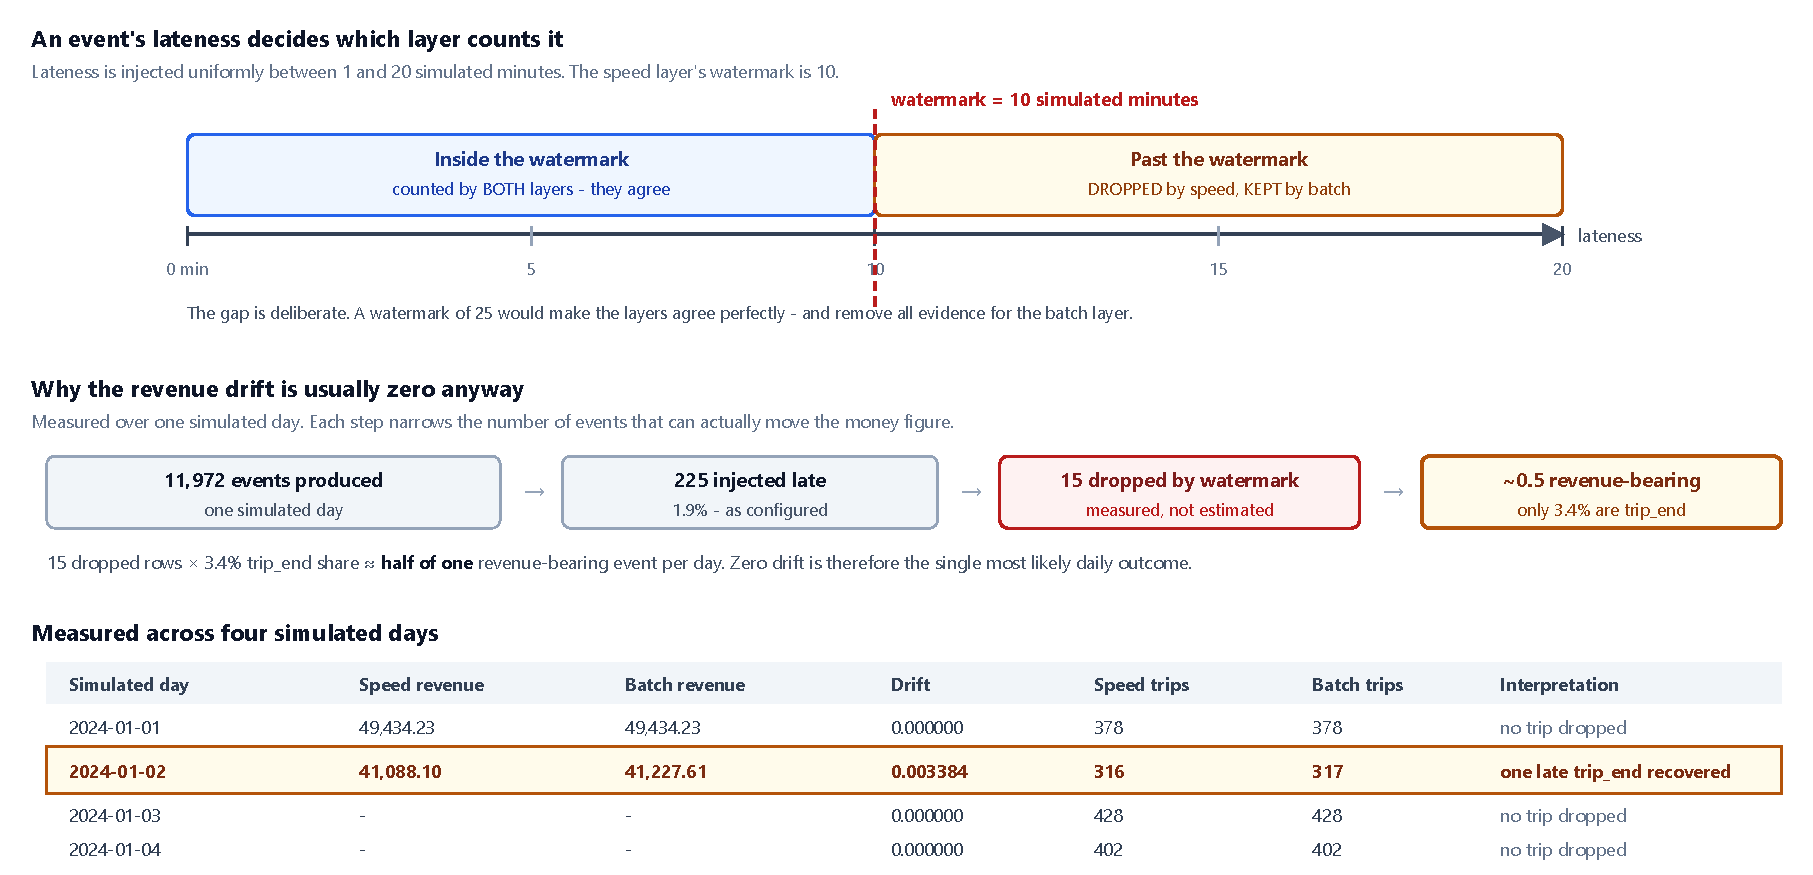
\includegraphics[width=0.9\textwidth]{figures/fig2-consistency.pdf}
\caption[Why the two layers disagree]{Why the two layers disagree: an
event's lateness decides which layer counts it.}
\label{fig:consistency}
\end{figure}

\begin{table}[htbp]
\centering
\caption{Reconciliation outcomes over four simulated days.}
\label{tab:four-days}
\begin{tabularx}{\textwidth}{@{}lRRRRR@{}}
\toprule
\textbf{Simulated day} & \textbf{Fleet margin} & \textbf{Unprof.} &
\textbf{Becoming unprof.} & \textbf{Dist. mismatch} &
\textbf{Revenue drift}\\
\midrule
2024-01-01 (partial) & 42.8\% & 6 & 0 & 2 & 0.000000\\
2024-01-02           & 38.3\% & 4 & 0 & 21 & \textbf{0.003384}\\
2024-01-03           & 45.8\% & 3 & 6 & 6 & 0.000000\\
2024-01-04           & 47.7\% & 4 & 7 & 4 & 0.000000\\
\bottomrule
\end{tabularx}
\end{table}

On 2024-01-02 the speed layer counted 316 trips against the batch
layer's 317: one late \code{trip\_end} dropped by the watermark and
recovered by the batch layer. Drift is usually zero because, per day, the
watermark drops about 15 rows and only 3.4\% of events are
\code{trip\_end}, so the expected number of lost revenue events is
$15 \times 0.034 \approx 0.5$. \code{fleet\_late\_rows\_dropped\_total}
therefore shows the \emph{mechanism} (reliably non-zero) and
\code{fleet\_speed\_batch\_drift\_ratio} its \emph{financial weight}
(usually zero). The case for batch-computed money is not that the speed
layer is badly wrong, but that its error is unbounded in principle, and
no watermark can absorb a correction arriving weeks later.

\section{Recomputation Demonstrated}
\label{sec:recompute}

Dropping a \code{v2} expense file for a reconciled day made it pending
again; the recompute produced \textbf{the same 50 rows with new values}
(net profit 19,770.78 $\rightarrow$ 21,177.99). A forced rerun of
2024-01-03 returned \textbf{bit-identical figures} (net 24,902.95). The
restatement came from one Parquet partition, with no log replay.

\section{Verification}
\label{sec:alerting-results}

\begin{itemize}
  \item 202 unit, PySpark and API tests pass; the smoke test passes 28/28
        checks; all 13 services start healthy from a fresh clone.
  \item 5 of 10 alert rules were observed firing \emph{and} delivered;
        \code{BatchRunFailed} is deliberately inhibited when
        \code{ExpenseFileLate} explains the same failure.
  \item 23 of 23 Grafana panel queries return live data.
  \item Batch task times: \code{compute\_vehicle\_day} 9.44\,s,
        \code{load\_batch\_views} 0.99\,s, all others under 0.5\,s.
\end{itemize}

\section{Discussion}
\label{sec:discussion}

\textbf{Defects found by operating the system.} \label{sec:defects}
Six defects surfaced only at runtime. The most
serious: a Spark worker restart killed the archiver's executor while the
query stayed ``active'', so the \textbf{healthcheck stayed green} while
nothing was archived for 26 minutes (fixed by a progress watchdog).
Others: an odometer checkpoint every 30 real seconds (30 simulated
minutes) that caused false distance mismatches; uncalibrated economics
flagging 35 of 50 vehicles unprofitable; batch gauges exported by every
service, firing a permanent false alert; an expense SLA applied to
corrected \code{v2} files; and two Windows-only start-up bugs.

\textbf{Limitations.} Four days is one run of one configuration, and
day~1 is partial. \code{becoming\_unprofitable} needs three reconciled
days to fire. Batch Spark runs in local mode and Kafka has a single
broker at RF~1. Because simulated time follows the wall clock, downtime
appears in the data as low demand.

\textbf{At production scale.} \label{sec:production}
Kafka would move to three brokers at RF~3 with a
schema registry (keeping the \code{vehicle\_id} key); the lake would use
object storage with a table format such as Iceberg or Delta and
compaction; processing would run on Kubernetes with the archiver
separated from the speed layer; and observability would add log
aggregation, tracing, and SLOs with ratio-based thresholds.

\chapter{Conclusions and Recommendations}
\label{ch:conclusion}

The brief's business question is really two questions, and their latency,
accuracy and recomputability requirements do not fit together. What
justifies Lambda here is not convention but one property Kappa cannot
supply cheaply: \textbf{restating a past day's financial figures when a
correction arrives on a different channel, days later.} We showed that
property working. A corrected file triggers an idempotent recompute
producing the same 50 rows with updated values, and a forced replay
returns bit-identical figures.

We also put a number on the speed layer's approximation instead of
asserting one, then explained arithmetically why it is as small as it is.
A measured drift of \code{0.000000} on three days of four, reported next
to the arithmetic that predicts it, beats a bigger number obtained by
quietly raising the fault rate. Lambda's usual weakness, two codebases
drifting apart, we answered with the shared \code{common/} package and
tests that hold its two duplications in step. For a reader who arrives
persuaded by Kreps, that is the part we would defend hardest.

\section*{Recommendations}

In priority order, and independent of scale:

\begin{enumerate}
  \item \textbf{Decouple the archiver from the speed layer} onto separate
        workers. They already have separate checkpoints; sharing cores is
        what turned a worker restart into 26 minutes of lost archiving.
  \item \textbf{Add a schema registry} in front of the telemetry topic,
        so a bad producer is rejected at publish time instead of
        discovered in the dead-letter queue, and give the DLQ an
        automated replay path.
  \item \textbf{Adopt a lake table format} (Iceberg or Delta Lake), to
        give lake writes the atomicity delete-then-insert already gives
        the PostgreSQL views.
  \item \textbf{Annotate outage windows}, so the
        \code{becoming\_unprofitable} rule can exclude degraded days
        instead of reading them as a commercial decline.
  \item \textbf{Express alert thresholds as ratios}, so that
        \code{IdleVehiclesHigh} survives a change in fleet size.
\end{enumerate}

% Two extra lines here keep the closing paragraph on the same page and the
% body inside the brief's 15-page guideline. The document is already
% \raggedbottom, so pages end at varying heights anyway.
\enlargethispage{2\baselineskip}
The most valuable thing we got out of this was not the architecture. It
was what running it turned up: a green healthcheck over a dead archiver,
a correct pipeline producing meaningless economics, an interval
60$\times$ longer than we intended. None of it visible in code review.


%====================================================================
% APPENDICES
%====================================================================
\appendix
{\small
\chapter{Alert Rule Inventory}
\label{app:alerts}

\begin{table}[htbp]
\centering
\caption{The ten Prometheus alert rules. \emph{Verified} means observed
firing \textbf{and} delivered into \code{alert\_notifications}.}
\label{tab:alerts}
\begin{tabularx}{\textwidth}{@{}lllXl@{}}
\toprule
\textbf{Alert} & \textbf{Stage} & \textbf{Sev.} & \textbf{Condition} &
\textbf{Verified}\\
\midrule
\code{TelemetryNotProduced} & ingestion & critical &
  No events produced for over a minute & yes\\
\code{DLQRateHigh} & ingestion & warning &
  More than 2\% of events dead-lettered & yes\\
\code{StreamStalled} & processing & critical &
  A named query has stopped progressing & --\\
\code{StreamLagHigh} & processing & warning &
  Query more than 5{,}000 offsets behind & --\\
\code{ExpenseFileLate} & orchestration & warning &
  Expense file missed its first-delivery SLA & yes\\
\code{BatchRunFailed} & orchestration & critical &
  Last reconciliation run failed & inhibited\\
\code{BatchNotRunRecently} & orchestration & warning &
  No successful reconciliation in 45 minutes & yes\\
\code{SpeedBatchDriftHigh} & processing & warning &
  Speed and batch revenue differ by over 5\% & --\\
\code{ApiDown} & serving & critical &
  The serving API is not reachable & yes\\
\code{IdleVehiclesHigh} & serving & warning &
  More than 8 vehicles idle past threshold & --\\
\bottomrule
\end{tabularx}
\end{table}

\chapter{API Surface}
\label{app:api}

\begin{table}[htbp]
\centering
\caption{The eleven documented endpoints, by the layer that answers
them.}
\label{tab:api}
\begin{tabularx}{\textwidth}{@{}llX@{}}
\toprule
\textbf{Endpoint} & \textbf{Layer} & \textbf{Answers}\\
\midrule
\code{GET /health} & ops & Liveness, \code{sim\_time}, compression\\
\code{GET /fleet/live} & speed & Active vehicles, idle ratio, trips/hour,
  earnings\\
\code{GET /zones/live} & speed & Current utilisation and earnings by zone\\
\code{GET /zones/\{id\}/hourly} & speed & One zone's hourly history\\
\code{GET /alerts/idle} & speed & Open and closed idle alerts\\
\code{GET /vehicles/unprofitable} & batch & Vehicles flagged
  (becoming) unprofitable\\
\code{GET /vehicles/\{id\}} & both & Labelled speed and batch blocks\\
\code{GET /reports/\{sim\_date\}} & batch & Daily reconciliation report\\
\code{GET /pipeline/status} & ops & Reconciled dates, last run, drift\\
\code{POST /alerts/webhook} & ops & Alertmanager delivery target\\
\code{GET /metrics} & ops & Prometheus exposition\\
\bottomrule
\end{tabularx}
\end{table}

\chapter{Statement of Individual Contributions}
\label{app:contributions}

Work was divided by \textbf{pipeline stage}, so each member owned one
vertical slice: its code, schema objects, tests and report sections.
Design decisions were taken jointly and code was reviewed across the
team.

\begin{table}[htbp]
\centering
\caption{Principal areas of responsibility by team member.}
\label{tab:contributions}
\begin{tabularx}{\textwidth}{@{}llX@{}}
\toprule
\textbf{Member} & \textbf{Reg. No.} & \textbf{Principal areas}\\
\midrule
Ahamed N.F.F. & EG/2021/4390 &
  Ingestion and data contract: \code{simulators/} (telemetry producer,
  fault injection, expense dropper), Kafka topics and partitioning, and
  the \code{simclock}, \code{schemas}, \code{validation}, \code{geo} and
  \code{earnings} modules of \code{common/}\\
\addlinespace
Safeer S.M. & EG/2021/4771 &
  Stream processing and serving: \code{streaming/} (archiver, speed
  layer, idle state machine, sinks, watchdog), \code{api/}, the
  \code{rt\_*} tables and the \code{db} helpers in \code{common/}\\
\addlinespace
Nafla M.N.P. & EG/2021/4687 &
  Batch, orchestration and observability: \code{batch/}, the
  \code{fleet\_daily\_reconciliation} DAG, \code{observability/}
  (Prometheus rules, Alertmanager, Grafana), and the
  \code{profitability}, \code{metrics} and \code{logging} modules of
  \code{common/}\\
\bottomrule
\end{tabularx}
\end{table}

Worked on jointly: \code{docs/SPEC.md}, \code{docker-compose.yml}, the
\code{Makefile}, the smoke test, the architecture and consistency
analysis, and every end-to-end acceptance run. A fuller breakdown is in
\code{docs/contributions.md}.

}

\end{document}
